\documentclass{article}

% content/resources/templates/preamble.tex
\usepackage[margin=0.6in]{geometry}
\author{Milav Dabgar}
\usepackage{amsmath,amssymb,amsthm}
\usepackage{booktabs}
\usepackage{multirow}
\usepackage{xcolor}
\usepackage{tcolorbox}
\tcbuselibrary{breakable,skins}
\usepackage[colorlinks=true,linkcolor=blue]{hyperref}
\usepackage{titlesec}
\usepackage{enumitem}
\usepackage{tikz}
\usepackage{pgfplots}
\usepackage{circuitikz}
\usepackage[version=4]{mhchem}
\usepackage{longtable}
\usepackage{array}
\usepackage{float}
\usepackage{caption}
\usepackage{listings}

\lstset{
  basicstyle=\small\ttfamily,
  breaklines=true,
  breakatwhitespace=false,
  postbreak=\mbox{\textcolor{red}{$\hookrightarrow$}\space},
  float=false,
  numbers=left,
  numberstyle=\tiny\color{gray},
  numbersep=10pt,
  xleftmargin=2em,
  keywordstyle=\color{blue},
  commentstyle=\color{green!60!black},
  stringstyle=\color{purple},
  backgroundcolor=\color{gray!5},
  showstringspaces=false,
  tabsize=2,
  captionpos=b,
  keepspaces=true,
  columns=flexible
}

\pgfplotsset{compat=1.18}
\usetikzlibrary{shapes,arrows,positioning,calc,patterns,decorations.pathmorphing,decorations.markings,arrows.meta}

% Color scheme
\definecolor{headcolor}{RGB}{0,102,204}
\definecolor{keycolor}{RGB}{220,20,60}
\definecolor{solutioncolor}{RGB}{34,139,34}
\definecolor{mnemoniccolor}{RGB}{148,0,211}
\definecolor{codecolor}{RGB}{0,0,100}

% Spacing
\setlength{\parskip}{3pt}
\setlist[itemize]{nosep}
\setlist[enumerate]{nosep}

% Title formatting
\titleformat{\section}{\Large\bfseries\color{headcolor}}{\thesection}{1em}{}
\titleformat{\subsection}{\large\bfseries\color{headcolor}}{\thesubsection}{1em}{}

% Pandoc tightlist compatibility
\providecommand{\tightlist}{%
  \setlength{\itemsep}{0pt}\setlength{\parskip}{0pt}}

% Pandoc longtable compatibility
\newcounter{none}
\def\thenone{}


% content/resources/templates/english-boxes.tex
% This file is currently empty - it exists to maintain consistency with the import structure.
% Add custom environments here if needed in the future.


% Custom commands for GTU solutions
% This file defines semantic commands for consistent formatting

% Question command with automatic formatting
\newcommand{\question}[2]{%
  \section*{Question #1}%
  \textbf{#2}%
}

% OR question variant
\newcommand{\questionor}[2]{%
  \section*{Question #1 OR}%
  \textbf{#2}%
}

% Proper table environment with caption
\newenvironment{answertable}[1]{%
  \begin{table}[htbp]
  \centering
  \caption{#1}
}{%
  \end{table}
}

% Proper figure environment for diagrams
\newenvironment{answerdiagram}[1]{%
  \begin{figure}[htbp]
  \centering
  \caption{#1}
}{%
  \end{figure}
}

% Semantic markup for key terms
\newcommand{\keyword}[1]{\textbf{#1}}
\newcommand{\code}[1]{\texttt{#1}}
\newcommand{\classname}[1]{\texttt{#1}}
\newcommand{\methodname}[1]{\texttt{#1}}

% Proper quotation marks
\newcommand{\mnemonic}[1]{``#1''}


\title{Digital Electronics (4321102) - Winter 2023 Solution}
\date{January 18, 2023}

\begin{document}
\maketitle

\questionmarks{1}{a}{3}
\textbf{(726)$_{10}$ = (\_\_\_\_\_\_\_\_\_)$_{2}$}

\begin{solutionbox}
\textbf{Answer}:

\captionof{table}{Decimal to Binary Conversion}
\begin{center}
\begin{tabulary}{\linewidth}{c c c}
\hline
\textbf{Step} & \textbf{Calculation} & \textbf{Remainder} \\
\hline
1 & 726 $\div$ 2 = 363 & 0 \\
2 & 363 $\div$ 2 = 181 & 1 \\
3 & 181 $\div$ 2 = 90 & 1 \\
4 & 90 $\div$ 2 = 45 & 0 \\
5 & 45 $\div$ 2 = 22 & 1 \\
6 & 22 $\div$ 2 = 11 & 0 \\
7 & 11 $\div$ 2 = 5 & 1 \\
8 & 5 $\div$ 2 = 2 & 1 \\
9 & 2 $\div$ 2 = 1 & 0 \\
10 & 1 $\div$ 2 = 0 & 1 \\
\hline
\end{tabulary}
\end{center}

Reading from bottom to top: (726)$_{10}$ = (1011010110)$_{2}$

\mnemonicbox{Divide By Two, Read Remainders Up}
\end{solutionbox}

\questionmarks{1}{b}{4}
\textbf{1) Convert binary number (10110101)$_{2}$ into gray number.}\\
\textbf{2) Convert gray number (10110110)$_{gray}$ into binary number.}

\begin{solutionbox}
\textbf{Answer}:

\textbf{Binary to Gray Conversion:}
\begin{lstlisting}
Binary:   1 0 1 1 0 1 0 1
           | | | | | | |
XOR:      1^0 0^1 1^1 1^0 0^1 1^0 0^1
           |   |   |   |   |   |   |
Gray:     1   1   0   1   1   1   1
\end{lstlisting}

Therefore: (10110101)$_{2}$ = (1101111)$_{gray}$

\textbf{Gray to Binary Conversion:}
\begin{lstlisting}
Gray:     1 0 1 1 0 1 1 0
           |
Binary:   1
          1^0 = 1
          1^1 = 0
          0^1 = 1
          1^0 = 1
          1^1 = 0
          0^1 = 1
          1^0 = 1
\end{lstlisting}

Therefore: (10110110)$_{gray}$ = (10110101)$_{2}$

\mnemonicbox{First bit same, rest XOR with previous binary}
\end{solutionbox}

\questionmarks{1}{c}{7}
\textbf{Explain NAND as a universal gate.}

\begin{solutionbox}
\textbf{Answer}:

\textbf{Diagram: NAND as Universal Gate}

\begin{center}
\begin{tikzpicture}[
    node distance=2cm,
    auto,
    block/.style={rectangle, draw, minimum width=1.5cm, minimum height=1cm, align=center},
    nand/.style={nand gate US, draw, logic gate inputs=nn}
]

% NOT using NAND
\node (A1) at (0,0) {A};
\node[nand, right of=A1, xshift=0.5cm] (N1) {};
\draw (A1) -- ++(0.5,0) |- (N1.input 1);
\draw (A1) -- ++(0.5,0) |- (N1.input 2);
\node[right of=N1] (Z1) {A'};
\draw (N1.output) -- (Z1);
\node[below=0.5cm of N1] {NOT Gate};

% AND using NAND
\node (A2) at (5,0.5) {A};
\node (B2) at (5,-0.5) {B};
\node[nand, right of=A2, yshift=-0.5cm, xshift=0.5cm] (N2) {};
\node[nand, right of=N2, xshift=0.5cm] (N3) {};
\draw (A2) -| (N2.input 1);
\draw (B2) -| (N2.input 2);
\draw (N2.output) -- ++(0.2,0) |- (N3.input 1);
\draw (N2.output) -- ++(0.2,0) |- (N3.input 2);
\node[right of=N3] (Z2) {A$\cdot$B};
\draw (N3.output) -- (Z2);
\node[below=0.5cm of N2, xshift=1cm] {AND Gate};

% OR using NAND
\node (A3) at (0,-3) {A};
\node (B3) at (0,-4) {B};
\node[nand, right of=A3, xshift=0.5cm] (N4) {};
\node[nand, right of=B3, xshift=0.5cm] (N5) {};
\node[nand, right of=N4, yshift=-0.5cm, xshift=1.5cm] (N6) {};

\draw (A3) -- ++(0.5,0) |- (N4.input 1);
\draw (A3) -- ++(0.5,0) |- (N4.input 2);
\draw (B3) -- ++(0.5,0) |- (N5.input 1);
\draw (B3) -- ++(0.5,0) |- (N5.input 2);

\draw (N4.output) -| (N6.input 1);
\draw (N5.output) -| (N6.input 2);

\node[right of=N6] (Z3) {A+B};
\draw (N6.output) -- (Z3);
\node[below=0.5cm of N6, xshift=-1cm] {OR Gate};

\end{tikzpicture}
\end{center}

\begin{itemize}
    \item \textbf{Universal Property}: NAND gate can implement any Boolean function without needing any other type of gate.
    \item \textbf{NOT Implementation}: Connecting both inputs of NAND together creates NOT gate.
    \item \textbf{AND Implementation}: NAND followed by another NAND creates AND gate.
    \item \textbf{OR Implementation}: Two NAND gates with single inputs, followed by NAND creates OR gate.
\end{itemize}

\captionof{table}{NAND Gate Implementations}
\begin{center}
\begin{tabulary}{\linewidth}{l l}
\hline
\textbf{Logic Function} & \textbf{NAND Implementation} \\
\hline
NOT(A) & NAND(A,A) \\
AND(A,B) & NAND(NAND(A,B),NAND(A,B)) \\
OR(A,B) & NAND(NAND(A,A),NAND(B,B)) \\
\hline
\end{tabulary}
\end{center}

\mnemonicbox{NAND can STAND as All gates}
\end{solutionbox}

\questionmarks{1}{c}{7}
\textbf{OR: Explain NOR as a universal gate.}

\begin{solutionbox}
\textbf{Answer}:

\textbf{Diagram: NOR as Universal Gate}

\begin{center}
\begin{tikzpicture}[
    node distance=2cm,
    auto,
    block/.style={rectangle, draw, minimum width=1.5cm, minimum height=1cm, align=center},
    nor/.style={nor gate US, draw, logic gate inputs=nn}
]

% NOT using NOR
\node (A1) at (0,0) {A};
\node[nor, right of=A1, xshift=0.5cm] (N1) {};
\draw (A1) -- ++(0.5,0) |- (N1.input 1);
\draw (A1) -- ++(0.5,0) |- (N1.input 2);
\node[right of=N1] (Z1) {A'};
\draw (N1.output) -- (Z1);
\node[below=0.5cm of N1] {NOT Gate};

% OR using NOR
\node (A2) at (5,0.5) {A};
\node (B2) at (5,-0.5) {B};
\node[nor, right of=A2, yshift=-0.5cm, xshift=0.5cm] (N2) {};
\node[nor, right of=N2, xshift=0.5cm] (N3) {};
\draw (A2) -| (N2.input 1);
\draw (B2) -| (N2.input 2);
\draw (N2.output) -- ++(0.2,0) |- (N3.input 1);
\draw (N2.output) -- ++(0.2,0) |- (N3.input 2);
\node[right of=N3] (Z2) {A+B};
\draw (N3.output) -- (Z2);
\node[below=0.5cm of N2, xshift=1cm] {OR Gate};

% AND using NOR
\node (A3) at (0,-3) {A};
\node (B3) at (0,-4) {B};
\node[nor, right of=A3, xshift=0.5cm] (N4) {};
\node[nor, right of=B3, xshift=0.5cm] (N5) {};
\node[nor, right of=N4, yshift=-0.5cm, xshift=1.5cm] (N6) {};

\draw (A3) -- ++(0.5,0) |- (N4.input 1);
\draw (A3) -- ++(0.5,0) |- (N4.input 2);
\draw (B3) -- ++(0.5,0) |- (N5.input 1);
\draw (B3) -- ++(0.5,0) |- (N5.input 2);

\draw (N4.output) -| (N6.input 1);
\draw (N5.output) -| (N6.input 2);

\node[right of=N6] (Z3) {A$\cdot$B};
\draw (N6.output) -- (Z3);
\node[below=0.5cm of N6, xshift=-1cm] {AND Gate};

\end{tikzpicture}
\end{center}

\begin{itemize}
    \item \textbf{Universal Property}: NOR gate can implement any Boolean function without needing any other type of gate.
    \item \textbf{NOT Implementation}: Connecting both inputs of NOR together creates NOT gate.
    \item \textbf{OR Implementation}: NOR followed by another NOR creates OR gate.
    \item \textbf{AND Implementation}: Two NOR gates with single inputs, followed by NOR creates AND gate.
\end{itemize}

\captionof{table}{NOR Gate Implementations}
\begin{center}
\begin{tabulary}{\linewidth}{l l}
\hline
\textbf{Logic Function} & \textbf{NOR Implementation} \\
\hline
NOT(A) & NOR(A,A) \\
OR(A,B) & NOR(NOR(A,B),NOR(A,B)) \\
AND(A,B) & NOR(NOR(A,A),NOR(B,B)) \\
\hline
\end{tabulary}
\end{center}

\mnemonicbox{NOR can form ALL logic cores}
\end{solutionbox}

\questionmarks{2}{a}{3}
\textbf{(11011011)$_{2}$ X (110)$_{2}$ = (\_\_\_\_\_\_\_\_\_)$_{2}$}

\begin{solutionbox}
\textbf{Answer}:

\captionof{table}{Binary Multiplication}
\begin{center}
\begin{lstlisting}
    1 1 0 1 1 0 1 1
  x         1 1 0
  ---------------
    0 0 0 0 0 0 0 0  (x 0)
  1 1 0 1 1 0 1 1    (x 1)
1 1 0 1 1 0 1 1      (x 1)
-----------------
1 0 0 0 0 0 0 1 1 0
\end{lstlisting}
\end{center}

Therefore: (11011011)$_{2}$ $\times$ (110)$_{2}$ = (10000001110)$_{2}$

\mnemonicbox{Multiply each bit, shift left, add all rows}
\end{solutionbox}

\questionmarks{2}{b}{4}
\textbf{Prove DeMorgan's theorem.}

\begin{solutionbox}
\textbf{Answer}:

\captionof{table}{DeMorgan's Theorem Proof}
\begin{center}
\begin{tabulary}{\linewidth}{c c c c c c c}
\hline
\textbf{A} & \textbf{B} & \textbf{A'} & \textbf{B'} & \textbf{A+B} & \textbf{(A+B)'} & \textbf{A'$\cdot$B'} \\
\hline
0 & 0 & 1 & 1 & 0 & 1 & 1 \\
0 & 1 & 1 & 0 & 1 & 0 & 0 \\
1 & 0 & 0 & 1 & 1 & 0 & 0 \\
1 & 1 & 0 & 0 & 1 & 0 & 0 \\
\hline
\end{tabulary}
\end{center}

\textbf{DeMorgan's Theorems:}
\begin{enumerate}
    \item $(A+B)' = A' \cdot B'$
    \item $(A \cdot B)' = A' + B'$
\end{enumerate}

Truth table proves that $(A+B)' = A' \cdot B'$ since both columns match.

\mnemonicbox{Break the line, change the sign}
\end{solutionbox}

\questionmarks{2}{c}{7}
\textbf{Explain full adder using logic circuit, Boolean equation and truth table.}

\begin{solutionbox}
\textbf{Answer}:

\textbf{Diagram: Full Adder Circuit}

\begin{center}
\begin{tikzpicture}[
    node distance=2.5cm,
    auto,
    block/.style={rectangle, draw, minimum width=1.5cm, minimum height=1cm, align=center}
]
    % Inputs
    \node (A) at (0, 2) {A};
    \node (B) at (0, 0) {B};
    \node (Cin) at (0, -2) {Cin};

    % Gates for Sum
    \node[xor gate US, draw, logic gate inputs=nn] (xor1) at (3, 1) {};
    \node[xor gate US, draw, logic gate inputs=nn] (xor2) at (6, 0) {};
    
    % Gates for Carry
    \node[and gate US, draw, logic gate inputs=nn] (and1) at (3, -1) {};
    \node[and gate US, draw, logic gate inputs=nn] (and2) at (3, -3) {};
    \node[and gate US, draw, logic gate inputs=nn] (and3) at (4.5, 3) {};  % A.B
    \node[or gate US, draw, logic gate inputs=nnn] (or1) at (7, -2) {};

    % Connections for Sum
    \draw (A) -| (xor1.input 1);
    \draw (B) -| (xor1.input 2);
    \draw (xor1.output) -- (xor2.input 1);
    \draw (Cin) -- ++(2,0) |- (xor2.input 2);
    \draw (xor2.output) -- ++(1,0) node[right] {Sum};

    % Connections for Carry
    \draw (A) |- (and3.input 1);
    \draw (B) |- (and3.input 2);
    
    \draw (B) |- (and1.input 1);
    \draw (Cin) |- (and1.input 2);
    
    \draw (A) to[out=0,in=180] ++(1,-3.5) |- (and2.input 1);
    \draw (Cin) to[out=0,in=180] ++(1,-0.5) |- (and2.input 2);

    \draw (and3.output) -| (or1.input 1);
    \draw (and1.output) -- (or1.input 2);
    \draw (and2.output) -| (or1.input 3);
    
    \draw (or1.output) -- ++(1,0) node[right] {Cout};

\end{tikzpicture}
\end{center}

\captionof{table}{Full Adder Truth Table}
\begin{center}
\begin{tabulary}{\linewidth}{c c c c c}
\hline
\textbf{A} & \textbf{B} & \textbf{Cin} & \textbf{Sum} & \textbf{Cout} \\
\hline
0 & 0 & 0 & 0 & 0 \\
0 & 0 & 1 & 1 & 0 \\
0 & 1 & 0 & 1 & 0 \\
0 & 1 & 1 & 0 & 1 \\
1 & 0 & 0 & 1 & 0 \\
1 & 0 & 1 & 0 & 1 \\
1 & 1 & 0 & 0 & 1 \\
1 & 1 & 1 & 1 & 1 \\
\hline
\end{tabulary}
\end{center}

\textbf{Boolean Equations}:
\begin{itemize}
    \item Sum = $A \oplus B \oplus Cin$
    \item Cout = $(A \cdot B) + (B \cdot Cin) + (A \cdot Cin)$
\end{itemize}

\mnemonicbox{Sum needs XOR three, Carry needs AND then OR}
\end{solutionbox}

\questionmarks{2}{a}{3}
\textbf{OR: Divide (11010010)$_{2}$ with (101)$_{2}$ = (\_\_\_\_\_\_\_\_\_)$_{2}$}

\begin{solutionbox}
\textbf{Answer}:

\captionof{table}{Binary Division}
\begin{center}
\begin{lstlisting}
            1 0 1 0 1 1
         ____________
1 0 1 ) 1 1 0 1 0 0 1 0
        1 0 1
        -----
          0 1 1
          0 0 0
          -----
            1 1 0
            1 0 1
            -----
              0 1 0
              0 0 0
              -----
                1 0 1
                1 0 1
                -----
                  0 0 0
\end{lstlisting}
\end{center}

Therefore: (11010010)$_{2}$ $\div$ (101)$_{2}$ = (101011)$_{2}$ with remainder (0)$_{2}$.

\mnemonicbox{Divide like decimal, but use binary subtraction}
\end{solutionbox}

\questionmarks{2}{b}{4}
\textbf{OR: Simplify the Boolean expression Y = A'B+AB'+A'B'+AB}

\begin{solutionbox}
\textbf{Answer}:

\captionof{table}{Boolean Simplification}
\begin{center}
\begin{tabulary}{\linewidth}{c l l}
\hline
\textbf{Step} & \textbf{Expression} & \textbf{Rule Applied} \\
\hline
1 & Y = A'B+AB'+A'B'+AB & Original \\
2 & Y = A'(B+B')+A(B'+B) & Factoring \\
3 & Y = A'(1)+A(1) & B+B' = 1 \\
4 & Y = A'+A & Simplifying \\
5 & Y = 1 & A'+A = 1 \\
\hline
\end{tabulary}
\end{center}

Therefore: Y = 1 (Always TRUE)

\mnemonicbox{Factor first, apply identities, combine like terms}
\end{solutionbox}

\questionmarks{2}{c}{7}
\textbf{OR: Explain full subtractor using logic circuit, boolean equation and truth table.}

\begin{solutionbox}
\textbf{Answer}:

\textbf{Diagram: Full Subtractor Circuit}

\begin{center}
\begin{tikzpicture}[
    node distance=2.5cm,
    auto,
    block/.style={rectangle, draw, minimum width=1.5cm, minimum height=1cm, align=center}
]
    % Inputs
    \node (A) at (0, 2) {A};
    \node (B) at (0, 0) {B};
    \node (Bin) at (0, -2) {Bin};

    % Gates for Difference
    \node[xor gate US, draw, logic gate inputs=nn] (xor1) at (3, 1) {};
    \node[xor gate US, draw, logic gate inputs=nn] (xor2) at (6, 0) {};
    
    % Gates for Borrow
    \node[not gate US, draw] (not1) at (1.5, 0.5) {}; 
    
    % Using logic for Bout = A'B + A'Bin + BBin
    \node[and gate US, draw, logic gate inputs=nn] (and1) at (4, -1.5) {}; 
    \node[and gate US, draw, logic gate inputs=nn] (and2) at (4, -3) {};
    \node[and gate US, draw, logic gate inputs=nn] (and3) at (4, 3) {};
    \node[or gate US, draw, logic gate inputs=nnn] (or1) at (7, -1) {};
    
    % Connections
    \draw (A) -| (xor1.input 1);
    \draw (B) -| (xor1.input 2);
    \draw (xor1.output) -- (xor2.input 1);
    \draw (Bin) -- ++(2,0) |- (xor2.input 2);
    \draw (xor2.output) -- ++(1,0) node[right] {Diff};
    
    \draw (A) -- ++(0.5,0) |- (not1.input);
    \draw (not1.output) -- ++(0.5,0) coordinate (notA);
    
    % A'B
    \draw (notA) |- (and3.input 1);
    \draw (B) |- (and3.input 2);
    
    % A'Bin
    \draw (notA) |- (and1.input 1);
    \draw (Bin) |- (and1.input 2);
    
    % BBin
    \draw (B) |- (and2.input 1);
    \draw (Bin) |- (and2.input 2);
    
    \draw (and3.output) -| (or1.input 1);
    \draw (and1.output) -- (or1.input 2);
    \draw (and2.output) -| (or1.input 3);
    
    \draw (or1.output) -- ++(1,0) node[right] {Bout};

\end{tikzpicture}
\end{center}

\captionof{table}{Full Subtractor Truth Table}
\begin{center}
\begin{tabulary}{\linewidth}{c c c c c}
\hline
\textbf{A} & \textbf{B} & \textbf{Bin} & \textbf{Difference} & \textbf{Bout} \\
\hline
0 & 0 & 0 & 0 & 0 \\
0 & 0 & 1 & 1 & 1 \\
0 & 1 & 0 & 1 & 1 \\
0 & 1 & 1 & 0 & 1 \\
1 & 0 & 0 & 1 & 0 \\
1 & 0 & 1 & 0 & 0 \\
1 & 1 & 0 & 0 & 0 \\
1 & 1 & 1 & 1 & 1 \\
\hline
\end{tabulary}
\end{center}

\textbf{Boolean Equations}:
\begin{itemize}
    \item Difference = $A \oplus B \oplus Bin$
    \item Bout = $(A' \cdot B) + (A' \cdot Bin) + (B \cdot Bin)$
\end{itemize}

\mnemonicbox{Difference uses triple XOR, Borrow when input is greater}
\end{solutionbox}

\questionmarks{3}{a}{3}
\textbf{Using 2's complement subtract (1011001)$_{2}$ from (1101101)$_{2}$.}

\begin{solutionbox}
\textbf{Answer}:

\captionof{table}{2's Complement Subtraction}
\begin{center}
\begin{tabulary}{\linewidth}{c l l}
\hline
\textbf{Step} & \textbf{Operation} & \textbf{Result} \\
\hline
1 & Number to subtract: & 1011001 \\
2 & 1's complement: & 0100110 \\
3 & 2's complement: & 0100111 \\
4 & (1101101) + (0100111) = & 10010100 \\
5 & Discard carry: & 0010100 \\
\hline
\end{tabulary}
\end{center}

Therefore: (1101101)$_{2}$ - (1011001)$_{2}$ = (0010100)$_{2}$ = (20)$_{10}$

\mnemonicbox{Flip bits, add one, then add numbers}
\end{solutionbox}

\questionmarks{3}{b}{4}
\textbf{Simplify Boolean equation using K-map: F(A,B,C,D) = $\Sigma$m(0,1,2,6,7,8,12,15)}

\begin{solutionbox}
\textbf{Answer}:

\textbf{Diagram: K-map Grouping}

\begin{center}
\begin{tikzpicture}
\matrix (map) [matrix of nodes,
               nodes={draw, minimum size=0.8cm, anchor=center},
               column sep=-\pgflinewidth,
               row sep=-\pgflinewidth]
{
1 & 1 & 0 & 1 \\
0 & 0 & 1 & 1 \\
1 & 0 & 1 & 0 \\
1 & 0 & 0 & 0 \\
};

\node[above=0.1cm] at (map-1-1.north west) {CD};
\node[left=0.1cm] at (map-1-1.north west) {AB};
\node[above] at (map-1-1.north) {00};
\node[above] at (map-1-2.north) {01};
\node[above] at (map-1-3.north) {11};
\node[above] at (map-1-4.north) {10};
\node[left] at (map-1-1.west) {00};
\node[left] at (map-2-1.west) {01};
\node[left] at (map-3-1.west) {11};
\node[left] at (map-4-1.west) {10};

\draw[red, rounded corners, thick] (map-1-1.north west) rectangle (map-1-2.south east);
\draw[red, rounded corners, thick] (map-4-1.north west) rectangle (map-4-1.south east);

\draw[blue, rounded corners, thick] (map-2-3.north west) rectangle (map-2-4.south east);
\draw[blue, rounded corners, thick] (map-3-3.north west) rectangle (map-3-3.south east);

\end{tikzpicture}
\end{center}

\begin{itemize}
    \item Group A: A'B'C' + A'B'CD' 
    \item Group B: BCD
    \item Group C: A'B'CD'
\end{itemize}

Simplified expression: F(A,B,C,D) = A'B'C' + BCD + A'B'CD'

\mnemonicbox{Find largest groups of 2\textsuperscript{n}, use minimal terms}
\end{solutionbox}

\questionmarks{3}{c}{7}
\textbf{Explain 3 to 8 decoder using logic circuit and truth table.}

\begin{solutionbox}
\textbf{Answer}:

\textbf{Diagram: 3-to-8 Decoder}

\begin{center}
\begin{tikzpicture}[
    node distance=1.5cm,
    auto,
    block/.style={rectangle, draw, minimum width=1.5cm, minimum height=1cm, align=center}
]
    % Inputs
    \node (A) at (0, 8) {A};
    \node (B) at (1, 8) {B};
    \node (C) at (2, 8) {C};
    
    % Inverters
    \node[not gate US, draw, rotate=-90] (notA) at (0.5, 7) {};
    \node[not gate US, draw, rotate=-90] (notB) at (1.5, 7) {};
    \node[not gate US, draw, rotate=-90] (notC) at (2.5, 7) {};
    
    \draw (A) |- (notA.input);
    \draw (B) |- (notB.input);
    \draw (C) |- (notC.input);
    
    % Lines down
    \draw (A) -- (0, -1);
    \draw (notA.output) -- (0.5, -1);
    \draw (B) -- (1, -1);
    \draw (notB.output) -- (1.5, -1);
    \draw (C) -- (2, -1);
    \draw (notC.output) -- (2.5, -1);
    
    % AND Gates
    \foreach \i in {0,1,2,3,4,5,6,7} {
        \node[and gate US, draw, logic gate inputs=nnn, scale=0.8] (and\i) at (5, 6.5-\i) {};
        \node[right] at (and\i.output) {D\i};
        \draw (and\i.output) -- ++(0.5,0);
    }
    
    % Connections
    \draw (0.5, 6.5) -- (and0.input 1);
    \draw (1.5, 6.5) -- (and0.input 2);
    \draw (2.5, 6.5) -- (and0.input 3);
    
    \draw (0, -0.5) -- (and7.input 1);
    \draw (1, -0.5) -- (and7.input 2);
    \draw (2, -0.5) -- (and7.input 3);
    
    \node at (3.5, 3) {Decoder Logic Array};

\end{tikzpicture}
\end{center}

\captionof{table}{3-to-8 Decoder Truth Table}
\begin{center}
\begin{tabulary}{\linewidth}{c c c c c c c c c c c}
\hline
\textbf{A} & \textbf{B} & \textbf{C} & \textbf{D0} & \textbf{D1} & \textbf{D2} & \textbf{D3} & \textbf{D4} & \textbf{D5} & \textbf{D6} & \textbf{D7} \\
\hline
0 & 0 & 0 & 1 & 0 & 0 & 0 & 0 & 0 & 0 & 0 \\
0 & 0 & 1 & 0 & 1 & 0 & 0 & 0 & 0 & 0 & 0 \\
0 & 1 & 0 & 0 & 0 & 1 & 0 & 0 & 0 & 0 & 0 \\
0 & 1 & 1 & 0 & 0 & 0 & 1 & 0 & 0 & 0 & 0 \\
1 & 0 & 0 & 0 & 0 & 0 & 0 & 1 & 0 & 0 & 0 \\
1 & 0 & 1 & 0 & 0 & 0 & 0 & 0 & 1 & 0 & 0 \\
1 & 1 & 0 & 0 & 0 & 0 & 0 & 0 & 0 & 1 & 0 \\
1 & 1 & 1 & 0 & 0 & 0 & 0 & 0 & 0 & 0 & 1 \\
\hline
\end{tabulary}
\end{center}

\textbf{Boolean Equations}: D0 = A'$\cdot$B'$\cdot$C', D1 = A'$\cdot$B'$\cdot$C, ... D7 = A$\cdot$B$\cdot$C

\mnemonicbox{One hot output at binary address}
\end{solutionbox}

\questionmarks{3}{a}{3}
\textbf{OR: Do as directed. 1) (101011010111)$_{2}$ = (\_\_\_\_\_\_\_\_\_)$_{8}$}

\begin{solutionbox}
\textbf{Answer}:

\captionof{table}{Binary to Octal Conversion}
\begin{center}
\begin{lstlisting}
Binary:    1 0 1 | 0 1 1 | 0 1 0 | 1 1 1
             |       |       |       |
Octal:       5       3       2       7
\end{lstlisting}
\end{center}

Therefore: (101011010111)$_{2}$ = (5327)$_{8}$

\mnemonicbox{Group by threes, right to left}
\end{solutionbox}

\questionmarks{3}{b}{4}
\textbf{OR: Simplify Boolean equation using K-map: F(A,B,C,D) = $\Sigma$m(1,3,5,7,8,9,10,11)}

\begin{solutionbox}
\textbf{Answer}:

\textbf{Diagram: K-map Grouping}

\begin{center}
\begin{tikzpicture}
\matrix (map) [matrix of nodes,
               nodes={draw, minimum size=0.8cm, anchor=center},
               column sep=-\pgflinewidth,
               row sep=-\pgflinewidth]
{
0 & 1 & 1 & 0 \\
0 & 1 & 1 & 0 \\
0 & 0 & 0 & 0 \\
1 & 1 & 1 & 1 \\
};

\node[above=0.1cm] at (map-1-1.north west) {CD};
\node[left=0.1cm] at (map-1-1.north west) {AB};
\node[above] at (map-1-1.north) {00};
\node[above] at (map-1-2.north) {01};
\node[above] at (map-1-3.north) {11};
\node[above] at (map-1-4.north) {10};
\node[left] at (map-1-1.west) {00};
\node[left] at (map-2-1.west) {01};
\node[left] at (map-3-1.west) {11};
\node[left] at (map-4-1.west) {10};

\draw[red, rounded corners, thick] (map-1-2.north west) rectangle (map-2-3.south east); 
\draw[blue, rounded corners, thick] (map-4-1.north west) rectangle (map-4-4.south east);

\end{tikzpicture}
\end{center}

\begin{itemize}
    \item Group A: A'D (Cells 1,3,5,7)
    \item Group B: AB' (Cells 8,9,10,11)
\end{itemize}

Simplified expression: F(A,B,C,D) = A'D + AB'

\mnemonicbox{Group powers of 2, minimize variables}
\end{solutionbox}

\questionmarks{3}{c}{7}
\textbf{OR: Explain 8 to 1 multiplexer using logic circuit and truth table.}

\begin{solutionbox}
\textbf{Answer}:

\textbf{Diagram: 8-to-1 Multiplexer}

\begin{center}
\begin{tikzpicture}[
    node distance=1.5cm,
    auto,
    block/.style={rectangle, draw, minimum width=1.5cm, minimum height=1cm, align=center}
]
    % Select Lines
    \node (S0) at (2, 0) {S0};
    \node (S1) at (3, 0) {S1};
    \node (S2) at (4, 0) {S2};
    
    % AND Gates
    \foreach \i in {0,1,2,3,4,5,6,7} {
        \node[and gate US, draw, logic gate inputs=nnnn, scale=0.7] (and\i) at (6, \i*0.8) {};
        \node[left] at (and\i.input 1) {D\i};
        \draw (and\i.input 1) -- ++(-0.5,0);
    }
    
    % OR Gate
    \node[or gate US, draw, logic gate inputs=nnnnnnnn, scale=1.5] (or1) at (9, 3) {};
    
    \foreach \i in {0,1,2,3,4,5,6,7} {
        \draw (and\i.output) -- (or1.input \i+1); 
    }
    
    \draw (or1.output) -- ++(1,0) node[right] {Y};
    
    \node at (6, -2) {Logic Circuit Structure};

\end{tikzpicture}
\end{center}

\captionof{table}{8-to-1 Multiplexer Truth Table}
\begin{center}
\begin{tabulary}{\linewidth}{c c c c}
\hline
\textbf{S2} & \textbf{S1} & \textbf{S0} & \textbf{Output Y} \\
\hline
0 & 0 & 0 & D0 \\
0 & 0 & 1 & D1 \\
0 & 1 & 0 & D2 \\
0 & 1 & 1 & D3 \\
1 & 0 & 0 & D4 \\
1 & 0 & 1 & D5 \\
1 & 1 & 0 & D6 \\
1 & 1 & 1 & D7 \\
\hline
\end{tabulary}
\end{center}

\textbf{Boolean Equation}: Y = S2'S1'S0'D0 + ... + S2S1S0D7

\mnemonicbox{Select bits route one input to output}
\end{solutionbox}

\questionmarks{4}{a}{3}
\textbf{Draw the logic circuit for binary to gray convertor.}

\begin{solutionbox}
\textbf{Answer}:

\textbf{Diagram: Binary to Gray Code Converter}

\begin{center}
\begin{tikzpicture}[
    node distance=1.5cm,
    auto,
    block/.style={rectangle, draw, minimum width=1.5cm, minimum height=1cm, align=center}
]
    % Inputs
    \node (B3) at (0, 3) {B3};
    \node (B2) at (0, 2) {B2};
    \node (B1) at (0, 1) {B1};
    \node (B0) at (0, 0) {B0};
    
    % Outputs
    \node (G3) at (5, 3) {G3};
    \node (G2) at (5, 2) {G2};
    \node (G1) at (5, 1) {G1};
    \node (G0) at (5, 0) {G0};
    
    % XOR Gates
    \node[xor gate US, draw, logic gate inputs=nn] (xor1) at (3, 2) {};
    \node[xor gate US, draw, logic gate inputs=nn] (xor2) at (3, 1) {};
    \node[xor gate US, draw, logic gate inputs=nn] (xor3) at (3, 0) {};
    
    % Connections
    \draw (B3) -- (G3);
    
    \draw (B3) -- ++(1,0) |- (xor1.input 1);
    \draw (B2) -- (xor1.input 2);
    \draw (xor1.output) -- (G2);
    
    \draw (B2) -- ++(0.5,0) |- (xor2.input 1);
    \draw (B1) -- (xor2.input 2);
    \draw (xor2.output) -- (G1);
    
    \draw (B1) -- ++(0.5,0) |- (xor3.input 1);
    \draw (B0) -- (xor3.input 2);
    \draw (xor3.output) -- (G0);

\end{tikzpicture}
\end{center}

\begin{itemize}
    \item \textbf{Binary Inputs}: B3, B2, B1, B0 (most to least significant bits)
    \item \textbf{Gray Outputs}: G3, G2, G1, G0 (most to least significant bits)
    \item \textbf{Conversion Rule}: G3 = B3, G2 = B3 $\oplus$ B2, G1 = B2 $\oplus$ B1, G0 = B1 $\oplus$ B0
\end{itemize}

\mnemonicbox{First bit same, rest XOR neighbors}
\end{solutionbox}

\questionmarks{4}{b}{4}
\textbf{Explain working of Serial in Serial out shift register.}

\begin{solutionbox}
\textbf{Answer}:

\textbf{Diagram: Serial-In Serial-Out Shift Register}

\begin{center}
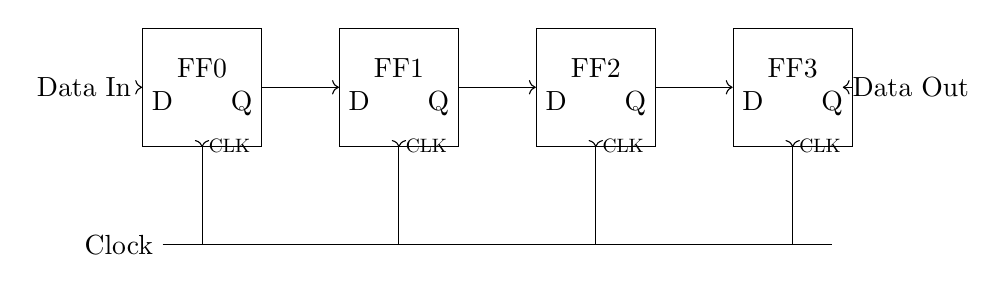
\begin{tikzpicture}[
    node distance=2cm,
    auto,
    block/.style={rectangle, draw, minimum width=1.5cm, minimum height=1.5cm, align=center}
]
    \foreach \i in {0,1,2,3} {
        \node[block] (FF\i) at (\i*2.5, 0) {FF\i\\D \hspace{0.5cm} Q};
        \draw[->] (\i*2.5, -1) -- (\i*2.5, -0.75) node[right, scale=0.7] {CLK} -- (FF\i.south);
    }
    
    \node (Din) at (-1.5, 0) {Data In};
    \draw[->] (Din) -- (FF0.west);
    
    \draw[->] (FF0.east) -- (FF1.west);
    \draw[->] (FF1.east) -- (FF2.west);
    \draw[->] (FF2.east) -- (FF3.west);
    
    \node (Dout) at (9, 0) {Data Out};
    \draw[->] (FF3.east) -- (Dout);
    
    % Clock Line
    \draw (-0.5, -2) node[left] {Clock} -- (8, -2);
    \foreach \i in {0,1,2,3} {
        \draw (\i*2.5, -2) -- (\i*2.5, -1);
    }

\end{tikzpicture}
\end{center}

\captionof{table}{Serial-In Serial-Out Operation}
\begin{center}
\begin{tabulary}{\linewidth}{c c c c c c}
\hline
\textbf{Clock Cycle} & \textbf{FF0} & \textbf{FF1} & \textbf{FF2} & \textbf{FF3} & \textbf{Data Out} \\
\hline
Initial & 0 & 0 & 0 & 0 & 0 \\
1 (Din=1) & 1 & 0 & 0 & 0 & 0 \\
2 (Din=0) & 0 & 1 & 0 & 0 & 0 \\
3 (Din=1) & 1 & 0 & 1 & 0 & 0 \\
4 (Din=1) & 1 & 1 & 0 & 1 & 1 \\
\hline
\end{tabulary}
\end{center}

\begin{itemize}
    \item \textbf{Operation}: Data bits enter serially at input, shift through all flip-flops, and exit serially.
    \item \textbf{Applications}: Data transmission, time delay, serial-to-serial conversion.
    \item \textbf{Features}: Simple design, requires fewer I/O pins but more clock cycles.
\end{itemize}

\mnemonicbox{One bit in, shift all, one bit out}
\end{solutionbox}

\questionmarks{4}{c}{7}
\textbf{Explain workings of D flip flop and JK flip flop using circuit diagram and truth table.}

\begin{solutionbox}
\textbf{Answer}:

\textbf{Diagram: D Flip-Flop}
\begin{center}
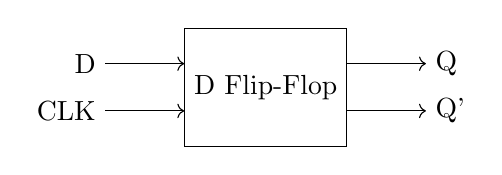
\begin{tikzpicture}[block/.style={rectangle, draw, minimum width=2cm, minimum height=1.5cm}]
    \node[block] (DFF) at (0,0) {D Flip-Flop};
    \draw[<-] (DFF.west) ++(0,0.3) -- ++(-1,0) node[left] {D};
    \draw[<-] (DFF.west) ++(0,-0.3) -- ++(-1,0) node[left] {CLK};
    \draw[->] (DFF.east) ++(0,0.3) -- ++(1,0) node[right] {Q};
    \draw[->] (DFF.east) ++(0,-0.3) -- ++(1,0) node[right] {Q'};
\end{tikzpicture}
\end{center}

\captionof{table}{D Flip-Flop Truth Table}
\begin{center}
\begin{tabulary}{\linewidth}{c c c}
\hline
\textbf{D} & \textbf{Clock} & \textbf{Q(next)} \\
\hline
0 & $\uparrow$ & 0 \\
1 & $\uparrow$ & 1 \\
\hline
\end{tabulary}
\end{center}

\textbf{Diagram: JK Flip-Flop}
\begin{center}
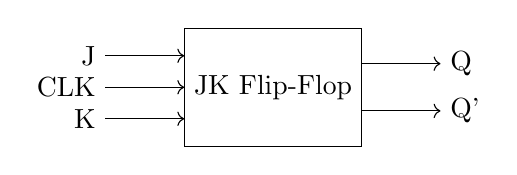
\begin{tikzpicture}[block/.style={rectangle, draw, minimum width=2cm, minimum height=1.5cm}]
    \node[block] (JKFF) at (0,0) {JK Flip-Flop};
    \draw[<-] (JKFF.west) ++(0,0.4) -- ++(-1,0) node[left] {J};
    \draw[<-] (JKFF.west) ++(0,0) -- ++(-1,0) node[left] {CLK};
    \draw[<-] (JKFF.west) ++(0,-0.4) -- ++(-1,0) node[left] {K};
    \draw[->] (JKFF.east) ++(0,0.3) -- ++(1,0) node[right] {Q};
    \draw[->] (JKFF.east) ++(0,-0.3) -- ++(1,0) node[right] {Q'};
\end{tikzpicture}
\end{center}

\captionof{table}{JK Flip-Flop Truth Table}
\begin{center}
\begin{tabulary}{\linewidth}{c c c c}
\hline
\textbf{J} & \textbf{K} & \textbf{Clock} & \textbf{Q(next)} \\
\hline
0 & 0 & $\uparrow$ & Q (no change) \\
0 & 1 & $\uparrow$ & 0 \\
1 & 0 & $\uparrow$ & 1 \\
1 & 1 & $\uparrow$ & Q' (toggle) \\
\hline
\end{tabulary}
\end{center}

\begin{itemize}
    \item \textbf{D Flip-Flop}: Data (D) input is transferred to output Q at positive clock edge.
    \item \textbf{JK Flip-Flop}: More versatile with set (J), reset (K), hold and toggle capabilities.
    \item \textbf{Applications}: Storage elements, counters, registers, sequential circuits.
\end{itemize}

\mnemonicbox{D Does what D is, JK Juggles Keep-Toggle-Set}
\end{solutionbox}

\questionmarks{4}{a}{3}
\textbf{OR: Draw the logic circuit for gray to binary convertor.}

\begin{solutionbox}
\textbf{Answer}:

\textbf{Diagram: Gray to Binary Code Converter}

\begin{center}
\begin{tikzpicture}[
    node distance=1.5cm,
    auto,
    block/.style={rectangle, draw, minimum width=1.5cm, minimum height=1cm, align=center}
]
    % Inputs
    \node (G3) at (0, 3) {G3};
    \node (G2) at (0, 2) {G2};
    \node (G1) at (0, 1) {G1};
    \node (G0) at (0, 0) {G0};
    
    % Outputs
    \node (B3) at (5, 3) {B3};
    \node (B2) at (5, 2) {B2};
    \node (B1) at (5, 1) {B1};
    \node (B0) at (5, 0) {B0};
    
    % XOR Gates
    \node[xor gate US, draw, logic gate inputs=nn] (xor1) at (3, 2) {};
    \node[xor gate US, draw, logic gate inputs=nn] (xor2) at (3, 1) {};
    \node[xor gate US, draw, logic gate inputs=nn] (xor3) at (3, 0) {};
    
    % Connections
    \draw (G3) -- (B3);
    
    \draw (G3) -- ++(1,0) -- ++(0,-0.5) -- ++(1.5,-0.5) |- (xor1.input 1); % Tricky wiring for G to B
    % Wait, rule: B3=G3. B2 = B3 xor G2. B1 = B2 xor G1.
    % So output B3 feeds into xor for B2.
    
    \draw (B3) ++(-1,0) -- ++(0,-0.5) |- (xor1.input 1); % From B3 line
    \draw (G2) -- (xor1.input 2);
    \draw (xor1.output) -- (B2);
    
    \draw (xor1.output) ++(0.5,0) -- ++(0,-0.5) |- (xor2.input 1);
    \draw (G1) -- (xor2.input 2);
    \draw (xor2.output) -- (B1);
    
    \draw (xor2.output) ++(0.5,0) -- ++(0,-0.5) |- (xor3.input 1);
    \draw (G0) -- (xor3.input 2);
    \draw (xor3.output) -- (B0);

\end{tikzpicture}
\end{center}

\begin{itemize}
    \item \textbf{Gray Inputs}: G3, G2, G1, G0
    \item \textbf{Binary Outputs}: B3, B2, B1, B0
    \item \textbf{Conversion Rule}: B3 = G3, B2 = B3 $\oplus$ G2, B1 = B2 $\oplus$ G1, B0 = B1 $\oplus$ G0
\end{itemize}

\mnemonicbox{First bit same, rest XOR with previous result}
\end{solutionbox}

\questionmarks{4}{b}{4}
\textbf{OR: Explain working of Parallel in Parallel out shift register.}

\begin{solutionbox}
\textbf{Answer}:

\textbf{Diagram: Parallel-In Parallel-Out Shift Register}

\begin{center}
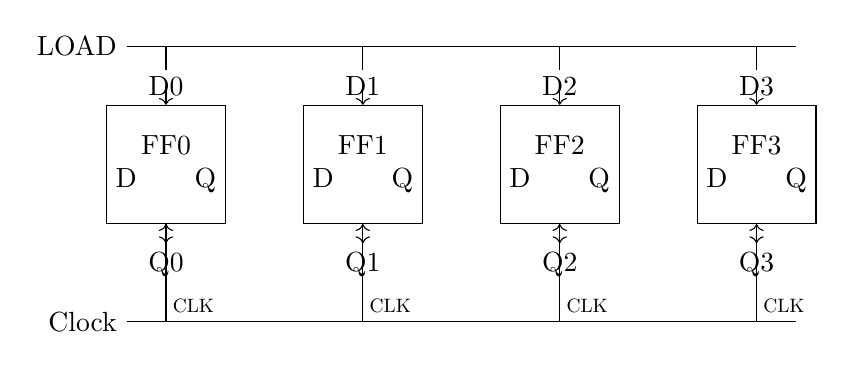
\begin{tikzpicture}[
    node distance=2cm,
    auto,
    block/.style={rectangle, draw, minimum width=1.5cm, minimum height=1.5cm, align=center}
]
    \foreach \i in {0,1,2,3} {
        \node[block] (FF\i) at (\i*2.5, 0) {FF\i\\D \hspace{0.5cm} Q};
        \node[above] at (FF\i.north) {D\i};
        \draw[->] (\i*2.5, 1) -- (FF\i.north);
        \draw[->] (FF\i.south) -- (\i*2.5, -1) node[below] {Q\i};
        \draw[->] (\i*2.5, -2) -- (\i*2.5, -1.8) node[right, scale=0.7] {CLK} -- (FF\i.south); % Visual clock
    }
    
    % Clock Line
    \draw (-0.5, -2) node[left] {Clock} -- (8, -2);
    
    % Load control (simplified as LOAD signal usually enables clock or D inputs)
    \draw (-0.5, 1.5) node[left] {LOAD} -- (8, 1.5);
    \foreach \i in {0,1,2,3} {
        \draw (\i*2.5, 1.5) -- (\i*2.5, 1.2);
    }

\end{tikzpicture}
\end{center}

\captionof{table}{Parallel-In Parallel-Out Operation}
\begin{center}
\begin{tabulary}{\linewidth}{c c c c}
\hline
\textbf{LOAD} & \textbf{Clock} & \textbf{D0-D3} & \textbf{Q0-Q3 (after clock)} \\
\hline
1 & $\uparrow$ & 1010 & 1010 \\
0 & $\uparrow$ & xxxx & 1010 (no change) \\
1 & $\uparrow$ & 0101 & 0101 \\
\hline
\end{tabulary}
\end{center}

\begin{itemize}
    \item \textbf{Operation}: Data loaded in parallel, all bits simultaneously transferred to outputs.
    \item \textbf{Applications}: Data storage, buffering, temporary holding registers.
    \item \textbf{Features}: Fastest register type, requires most I/O pins, no bit shifting.
\end{itemize}

\mnemonicbox{All in, all out, all at once}
\end{solutionbox}

\questionmarks{4}{c}{7}
\textbf{OR: Explain workings of T flip flop and SR flip flop using circuit diagram and truth table.}

\begin{solutionbox}
\textbf{Answer}:

\textbf{Diagram: T Flip-Flop}
\begin{center}
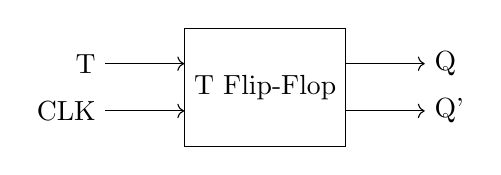
\begin{tikzpicture}[block/.style={rectangle, draw, minimum width=2cm, minimum height=1.5cm}]
    \node[block] (TFF) at (0,0) {T Flip-Flop};
    \draw[<-] (TFF.west) ++(0,0.3) -- ++(-1,0) node[left] {T};
    \draw[<-] (TFF.west) ++(0,-0.3) -- ++(-1,0) node[left] {CLK};
    \draw[->] (TFF.east) ++(0,0.3) -- ++(1,0) node[right] {Q};
    \draw[->] (TFF.east) ++(0,-0.3) -- ++(1,0) node[right] {Q'};
\end{tikzpicture}
\end{center}

\captionof{table}{T Flip-Flop Truth Table}
\begin{center}
\begin{tabulary}{\linewidth}{c c c}
\hline
\textbf{T} & \textbf{Clock} & \textbf{Q(next)} \\
\hline
0 & $\uparrow$ & Q (no change) \\
1 & $\uparrow$ & Q' (toggle) \\
\hline
\end{tabulary}
\end{center}

\textbf{Diagram: SR Flip-Flop}
\begin{center}
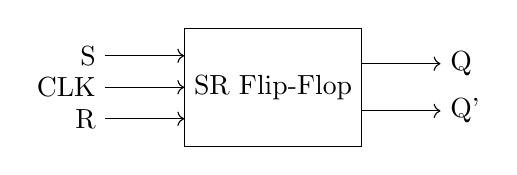
\begin{tikzpicture}[block/.style={rectangle, draw, minimum width=2cm, minimum height=1.5cm}]
    \node[block] (SRFF) at (0,0) {SR Flip-Flop};
    \draw[<-] (SRFF.west) ++(0,0.4) -- ++(-1,0) node[left] {S};
    \draw[<-] (SRFF.west) ++(0,0) -- ++(-1,0) node[left] {CLK};
    \draw[<-] (SRFF.west) ++(0,-0.4) -- ++(-1,0) node[left] {R};
    \draw[->] (SRFF.east) ++(0,0.3) -- ++(1,0) node[right] {Q};
    \draw[->] (SRFF.east) ++(0,-0.3) -- ++(1,0) node[right] {Q'};
\end{tikzpicture}
\end{center}

\captionof{table}{SR Flip-Flop Truth Table}
\begin{center}
\begin{tabulary}{\linewidth}{c c c c}
\hline
\textbf{S} & \textbf{R} & \textbf{Clock} & \textbf{Q(next)} \\
\hline
0 & 0 & $\uparrow$ & Q (no change) \\
0 & 1 & $\uparrow$ & 0 (reset) \\
1 & 0 & $\uparrow$ & 1 (set) \\
1 & 1 & $\uparrow$ & Invalid \\
\hline
\end{tabulary}
\end{center}

\begin{itemize}
    \item \textbf{T Flip-Flop}: Toggle flip-flop changes state when T=1, maintains state when T=0.
    \item \textbf{SR Flip-Flop}: Basic flip-flop with Set (S) and Reset (R) inputs.
    \item \textbf{Applications}: T flip-flops for counters and frequency dividers, SR for basic memory.
\end{itemize}

\mnemonicbox{T Toggles when True, SR Sets or Resets}
\end{solutionbox}

\questionmarks{5}{a}{3}
\textbf{Compare TTL, CMOS and ECL logic families.}

\begin{solutionbox}
\textbf{Answer}:

\captionof{table}{Comparison of Logic Families}
\begin{center}
\begin{tabulary}{\linewidth}{l l l l}
\hline
\textbf{Parameter} & \textbf{TTL} & \textbf{CMOS} & \textbf{ECL} \\
\hline
Power Consumption & Medium & Very Low & High \\
Speed & Medium & Low-Medium & Very High \\
Noise Immunity & Medium & High & Low \\
Fan-out & 10 & $>$50 & 25 \\
Supply Voltage & +5V & +3V to +15V & -5.2V \\
Complexity & Medium & Low & High \\
\hline
\end{tabulary}
\end{center}

\begin{itemize}
    \item \textbf{TTL}: Transistor-Transistor Logic - Good balance of speed and power.
    \item \textbf{CMOS}: Complementary Metal-Oxide-Semiconductor - Low power, high density.
    \item \textbf{ECL}: Emitter-Coupled Logic - Highest speed, used in high-performance applications.
\end{itemize}

\mnemonicbox{TCE: TTL Compromises, CMOS Economizes, ECL Excels in speed}
\end{solutionbox}

\questionmarks{5}{b}{4}
\textbf{Explain decade counter with the help of logic circuit diagram and truth table.}

\begin{solutionbox}
\textbf{Answer}:

\textbf{Diagram: Decade Counter (BCD Counter)}

\begin{center}
\begin{tikzpicture}[
    node distance=2.5cm,
    auto,
    block/.style={rectangle, draw, minimum width=1.5cm, minimum height=1.5cm, align=center}
]
    \foreach \i in {0,1,2,3} {
        \node[block] (JK\i) at (\i*2.8, 0) {JK FF\i\\J \hspace{0.5cm} K};
        \draw (\JK\i) -- ++(0,1) node[above] {Q\i}; % Node placement fix needed
        \node at (\i*2.8, 1) {Q\i};
    }
    % Simplified connections representation for complexity management
    \node at (4.5, -2) {Logic: JK Flip-Flops cascaded with NAND reset logic at 1010 (10)};
    \draw (0, -1) -- (8.5, -1) node[right] {Common Clock/Control};

\end{tikzpicture}
\end{center}

\captionof{table}{Decade Counter States}
\begin{center}
\begin{tabulary}{\linewidth}{c c c c c}
\hline
\textbf{Count} & \textbf{Q3} & \textbf{Q2} & \textbf{Q1} & \textbf{Q0} \\
\hline
0 & 0 & 0 & 0 & 0 \\
1 & 0 & 0 & 0 & 1 \\
2 & 0 & 0 & 1 & 0 \\
3 & 0 & 0 & 1 & 1 \\
4 & 0 & 1 & 0 & 0 \\
5 & 0 & 1 & 0 & 1 \\
6 & 0 & 1 & 1 & 0 \\
7 & 0 & 1 & 1 & 1 \\
8 & 1 & 0 & 0 & 0 \\
9 & 1 & 0 & 0 & 1 \\
0 & 0 & 0 & 0 & 0 \\
\hline
\end{tabulary}
\end{center}

\begin{itemize}
    \item \textbf{Function}: Counts from 0 to 9 (decimal) and then resets to 0.
    \item \textbf{Applications}: Digital clocks, frequency dividers, BCD counters.
    \item \textbf{Features}: Auto-reset at count 10, synchronous with clock.
\end{itemize}

\mnemonicbox{Counts one Decade, resets after nine}
\end{solutionbox}

\questionmarks{5}{c}{7}
\textbf{Give Classification of Memories in detail.}

\begin{solutionbox}
\textbf{Answer}:

\textbf{Diagram: Memory Classification}

\begin{center}
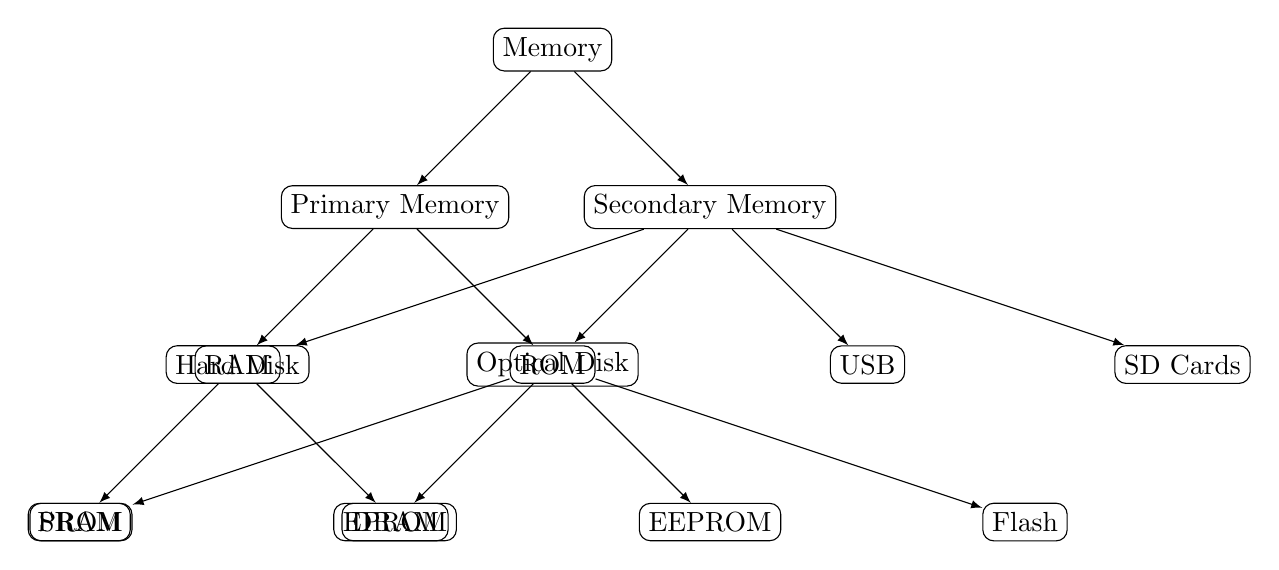
\begin{tikzpicture}[
    edge from parent/.style={draw, -latex},
    sibling distance=4cm,
    level distance=2cm,
    every node/.style={rectangle, draw, rounded corners, align=center}
]
\node {Memory}
    child { node {Primary Memory}
        child { node {RAM}
            child { node {SRAM} }
            child { node {DRAM} }
        }
        child { node {ROM}
            child { node {PROM} }
            child { node {EPROM} }
            child { node {EEPROM} }
            child { node {Flash} }
        }
    }
    child { node {Secondary Memory}
        child { node {Hard Disk} }
        child { node {Optical Disk} }
        child { node {USB} }
        child { node {SD Cards} }
    };
\end{tikzpicture}
\end{center}

\captionof{table}{Memory Types Comparison}
\begin{center}
\begin{tabulary}{\linewidth}{l l l l l}
\hline
\textbf{Memory Type} & \textbf{Volatility} & \textbf{Read/Write} & \textbf{Access Speed} & \textbf{Typical Use} \\
\hline
SRAM & Volatile & R/W & Very Fast & Cache memory \\
DRAM & Volatile & R/W & Fast & Main memory \\
ROM & Non-volatile & Read-only & Medium & BIOS, firmware \\
PROM & Non-volatile & Write-once & Medium & Permanent programs \\
EPROM & Non-volatile & Erasable UV & Medium & Upgradable firmware \\
EEPROM & Non-volatile & Electrically & Medium & Configuration data \\
Flash & Non-volatile & Block erasable & Medium-Fast & Storage devices \\
\hline
\end{tabulary}
\end{center}

\begin{itemize}
    \item \textbf{RAM (Random Access Memory)}: Temporary, volatile working memory.
    \item \textbf{ROM (Read Only Memory)}: Permanent, non-volatile program storage.
\end{itemize}

\mnemonicbox{RAM Vanishes, ROM Remains}
\end{solutionbox}

\questionmarks{5}{a}{3}
\textbf{OR: Define: Fan out, Fan in and Figure of merit.}

\begin{solutionbox}
\textbf{Answer}:

\captionof{table}{Digital Logic Parameters}
\begin{center}
\begin{tabulary}{\linewidth}{l L l}
\hline
\textbf{Parameter} & \textbf{Definition} & \textbf{Typical Values} \\
\hline
Fan-out & Number of standard loads a gate output can drive & TTL: 10, CMOS: $>$50 \\
Fan-in & Number of inputs a logic gate can handle & TTL: 8, CMOS: 100+ \\
Figure of Merit & Speed-power product (propagation delay $\times$ power consumption) & Lower is better \\
\hline
\end{tabulary}
\end{center}

\begin{itemize}
    \item \textbf{Fan-out}: Maximum number of gate inputs that can be connected to a gate output.
    \item \textbf{Fan-in}: Maximum number of inputs available on a single logic gate.
    \item \textbf{Figure of Merit}: Quality factor for comparing different logic families.
\end{itemize}

\mnemonicbox{Out drives many, In accepts many, Merit measures goodness}
\end{solutionbox}

\questionmarks{5}{b}{4}
\textbf{OR: Explain asynchronous up counter with the help of logic circuit diagram and truth table.}

\begin{solutionbox}
\textbf{Answer}:

\textbf{Diagram: 4-bit Asynchronous Up Counter}

\begin{center}
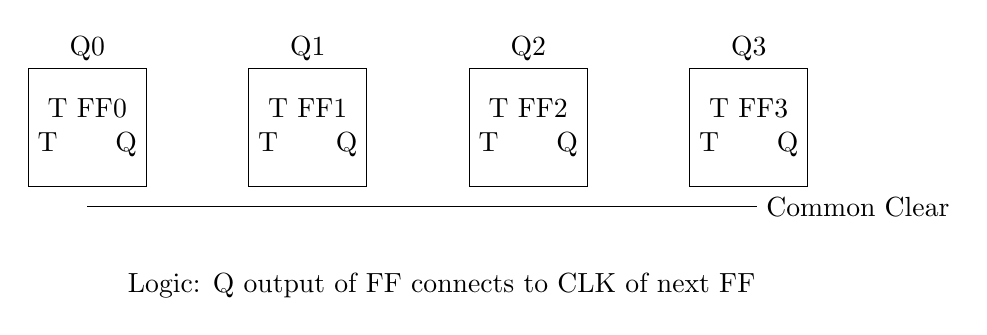
\begin{tikzpicture}[
    node distance=2.5cm,
    auto,
    block/.style={rectangle, draw, minimum width=1.5cm, minimum height=1.5cm, align=center}
]
    \foreach \i in {0,1,2,3} {
        \node[block] (TFF\i) at (\i*2.8, 0) {T FF\i\\T \hspace{0.5cm} Q};
        \node at (\i*2.8, 1) {Q\i};
    }
    
    \node at (4.5, -2) {Logic: Q output of FF connects to CLK of next FF};
    \draw (0, -1) -- (8.5, -1) node[right] {Common Clear};

\end{tikzpicture}
\end{center}

\captionof{table}{4-bit Asynchronous Counter States}
\begin{center}
\begin{tabulary}{\linewidth}{c c c c c}
\hline
\textbf{Count} & \textbf{Q3} & \textbf{Q2} & \textbf{Q1} & \textbf{Q0} \\
\hline
0 & 0 & 0 & 0 & 0 \\
1 & 0 & 0 & 0 & 1 \\
2 & 0 & 0 & 1 & 0 \\
... & .. & .. & .. & .. \\
14 & 1 & 1 & 1 & 0 \\
15 & 1 & 1 & 1 & 1 \\
\hline
\end{tabulary}
\end{center}

\begin{itemize}
    \item \textbf{Operation}: Each flip-flop triggers the next when transitioning from 1 to 0.
    \item \textbf{Features}: Simple design but suffers from propagation delay (ripple).
    \item \textbf{Applications}: Frequency division, basic counting applications.
\end{itemize}

\mnemonicbox{Ripples Up, Each bit triggers Next}
\end{solutionbox}

\questionmarks{5}{c}{7}
\textbf{OR: Describe steps and the need of E-waste Management of Digital ICs.}

\begin{solutionbox}
\textbf{Answer}:

\textbf{Diagram: E-waste Management Cycle}

\begin{center}
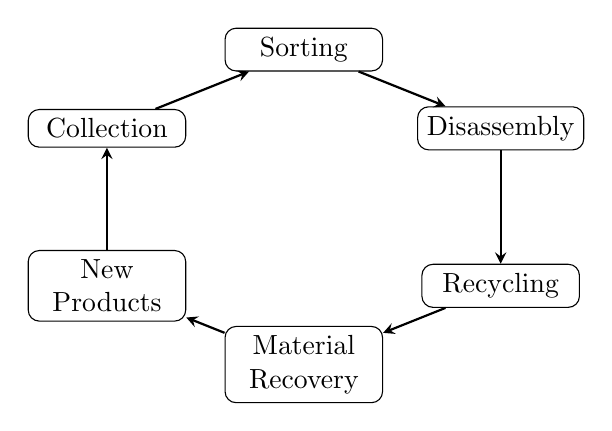
\begin{tikzpicture}[
    node distance=2cm,
    auto,
    block/.style={rectangle, draw, rounded corners, minimum width=2cm, align=center},
    arrow/.style={thick, ->, >=stealth}
]
    \node[block] (C) at (0, 0) {Collection};
    \node[block] (S) at (2.5, 1) {Sorting};
    \node[block] (D) at (5, 0) {Disassembly};
    \node[block] (R) at (5, -2) {Recycling};
    \node[block] (M) at (2.5, -3) {Material\\Recovery};
    \node[block] (N) at (0, -2) {New\\Products};
    
    \draw[arrow] (C) -- (S);
    \draw[arrow] (S) -- (D);
    \draw[arrow] (D) -- (R);
    \draw[arrow] (R) -- (M);
    \draw[arrow] (M) -- (N);
    \draw[arrow] (N) -- (C);

\end{tikzpicture}
\end{center}

\captionof{table}{E-waste Management Steps}
\begin{center}
\begin{tabulary}{\linewidth}{l l l}
\hline
\textbf{Step} & \textbf{Description} & \textbf{Importance} \\
\hline
Collection & Gathering obsolete ICs & Prevents improper disposal \\
Sorting & Categorizing by type & Enables efficient processing \\
Disassembly & Separating components & Facilitates material recovery \\
Recycling & Processing materials & Reduces environmental impact \\
Material Recovery & Extracting valuable metals & Conserves resources \\
Safe Disposal & Handling toxic components & Prevents contamination \\
\hline
\end{tabulary}
\end{center}

\begin{itemize}
    \item \textbf{Need for E-waste Management}:
    \begin{itemize}
        \item \textbf{Environmental Protection}: Prevents toxic substances from leaching into soil/water.
        \item \textbf{Resource Conservation}: Recovers valuable metals like gold, silver, copper.
        \item \textbf{Health Safety}: Reduces exposure to hazardous materials like lead, mercury.
        \item \textbf{Legal Compliance}: Follows regulations regarding electronic waste.
    \end{itemize}
\end{itemize}

\mnemonicbox{Collect, Sort, Disassemble, Recycle, Recover, Reuse}
\end{solutionbox}

\end{document}


